\documentclass[twoside]{article}
\usepackage{amssymb}
\usepackage{amsmath}
\usepackage{amsthm}
\usepackage{algorithm}
\usepackage{algpseudocode}
\usepackage{enumerate}% http://ctan.org/pkg/enumerate
\usepackage{pgfplots}
\usepackage{multicol}
\usepackage[hmarginratio=1:1,top=32mm,columnsep=20pt]{geometry}
\usepackage{fullpage}
\usepackage{pdflscape}
\usepackage{setspace}
\usepackage{tikz}
\usepackage[toc,page]{appendix}
\usepackage[shortlabels]{enumitem}\usepackage{draftwatermark}

\newcommand{\quotes}[1]{``#1''}

\theoremstyle{plain}% default
\newtheorem{theorem}{Theorem}[section]
\newtheorem{lemma}[theorem]{Lemma}
\newtheorem{proposition}[theorem]{Proposition}
\newtheorem*{corollary}{Corollary}

\theoremstyle{definition}
\newtheorem{definition}{Definition}[section]
\newtheorem{example}{Example}[section]
\newtheorem{exercise}[example]{Exercise}

\theoremstyle{remark}
\newtheorem*{rem}{Remark}
\newtheorem*{note}{Note}
\newtheorem{case}{Case}

\begin{document}
\parindent=0in
\parskip=12pt

\SetWatermarkText{Draft}
\SetWatermarkScale{5}

\title{
  Relative Probability on Finite Sample Spaces \\
  \large{
    SUBTITLE HERE
  }
}

\author{Max Sklar\\ Local Maximum Labs \\ DATE HERE}
\date{}

\maketitle
\thispagestyle{empty}

\begin{abstract}
This is an incomplete draft/outline of an upcoming paper. Please do not share
\end{abstract}

\tableofcontents
\newpage

\section{Introduction}

The mathematical foundations of probability theory are still very much open to debate!

Since Kolmogorov published the standard axioms for probability in 1933\cite{Kolmogorov}, there have been calls to relax or alter them for various applications. In Kolmogorov's Axiomatisation and Its Discontents\cite{lyon}, Lyon lays out these cases and their justifications. A question arises from this discuttion: can we discuss conditional probability when the condition event has probability zero? One would hope it not be forbidden to talk about the probability of an event given a hypothetical situation which will not occur\footnote{Another unintuitive feature of probability theory is that zero probability events do indeed occur, particularly when given a continuous distribution.}. Related to this question is whether we can talk about the relative probability of two events in a system, even though those two events may have probability zero.

The Kolmogorov model defines these values as a ratio of one probability to another. As a result, every time the indeterminate form \(\frac{0}{0}\) appears, the relative probability remains undefined. Undeterred by this state of affairs, mathematicians and engineers refer to this type of relative probability all the time. For example, if we consider the continuous probability distributrion over \([0, 1]\) given by the probability distribution function \(2x\), we know that the PDF at \(x = \frac{1}{2}\) is twice as much as the PDF at \(x = \frac{1}{4}\). In a sense, we believe that the former is twice as likely as the latter - even though we are only talking about \textit{probability density} or \textit{PDF} values.

Let us take the position that we may model probability in a non-standard way, and we can do so as long our new framework is logically consistent, and that the advertised applications correspond to the mathematical model\footnote{Lyon identifies this link between application and model as the bridge principle. A new set of axioms for probability could well give rise to a new and interesting mathematics, but if that mathematics cannot be linked to any application that anyone would reasonbly call probability, then it ought to go by a different name.}. Given the popularity of Bayesian methods as applied to machine learning in recent decades, and given that the methods used to search a hypothesis space in Bayesian inference relies on relative probability\cite{sklar_bias}, we ought to understand whether we can derive a framework for probability that takes the relationships between outcomes and events as fundamental.

This improves the Kolmogorov model - that takes absolute probability as fundamental - by both solving the conditional probability question and giving rise to new concepts and constructions to study.

\subsection{Goals}

A relative probability approach is not only viable, but has many properties that practicioners will find attractive.

As a proof of this concept, we will construct a theory of relative probability on finite distributions. By omitting infinite distributions, we can temporarily set aside the concepts of measurable sets and countable additivity. This work will demonstrate that even with this vast simplification there is much to be learned. Relative probability requires a new set of fundamental rules and vocabulary to be a viable foundation, which we will construct.

These methods have applications in Bayesian statistics, even providing a new formulation of Bayes rule that is reflective of current practice. We will look at these applications of these ideas along with their algorithmic implementation.

Finally, we discuss a critical feature of relative probability functions,
which is their ability to retain information when taking limits\textemdash for which absolute probability fails. In order to certify this feature, we delve into the topology and finish with a proof of compactness.

\section{Preliminaries}
\subsection{Magnitude Space}
\begin{definition}
The \textit{magnitude space} \(\mathbb{M}\) is the set of all positive real numbers, \(0\) and \(\infty\).
\[\mathbb{M} = [0, +\infty]\]
\end{definition}

Magnitudes roughly corresponding with our intuition of size.

\(\mathbb{M}\) is closed under addition with \(m + \infty = \infty\).

The products \(0 \cdot \infty\) and \(\infty \cdot 0\) are indeterminate. In all other cases, multiplication on \(\mathbb{M}\) is defined.

The multiplicative inverse \(m^{-1}\) is the defined on all \(\mathbb{M}\). We let \(0^{-1} := \infty\) and \(\infty^{-1} := 0\), even though it doesn't quite act as a multiplicative inverse in those cases.

The set of magnitudes is a totally ordered set under \(\leq\), meaning that for every two magnitudes either \(m_1 \leq m_2\) or \(m_2 \leq m_1\), and if both are true then \(m_1 = m_2\). The point at infinity can be considered a limit element, larger than all other magnitudes.

\subsection{The Wildcard Element}

\begin{definition}
Let the \textit{magnitude-wildcard space} \(\mathbb{M}^*= \mathbb{M} \cup \{\ast\}\) be the set of magnitudes along with a \textit{wildcard element}, \(\ast\).
\end{definition}

The wildcard element corresponds to several different concepts, each appearing in a different type of practice:
\begin{itemize}
  \item The \textit{wildcard pattern} used in pattern matching and regular expressions in type theory and computer science
  \item The indeterminate form \(\frac{0}{0}\) in arithmetic.
  \item The standard \textit{NaN}, or \textit{Not a Number}\footnote{\quotes{Not a Number} may have been an unfortunate naming choice because it actually represents \textbf{any} number!} value in the IEEE standard for floating point arithmetic\cite{ieee}.
\end{itemize}

The following properties on \(\ast\) to allow addition and multiplication of any two magnitude-wildcard values.
\begin{enumerate}[(i)]
  \item \(0 \cdot \infty = \ast\)
  \item \(\ast + m = \ast\)
  \item \(\ast \cdot m = \ast\)
\end{enumerate}

Note that we now lose some basic properties of these operations. For example, we can no longer simplfy an expression like \(0x\) to \(0\). This will take some getting used to, but programmers familiar with the \textit{NaN} value in floating point arithmetic have long adapted to this.

\subsection{The Matching Relation}

\begin{definition}
The \textit{matching relation}\footnote{It helps to read \(:\cong\) as \quotes{is matched by}.} \(:\cong\) is a binary relation on \(\mathbb{M}^*\). \(m_1\) is matched by \(m_2\) when either \(m_1 = m_2\) or  \(m_2\) is the wildcard.
\[m_1 :\cong m_2 \Longleftrightarrow (m_1 = m_1) \vee (m_2 = \ast)\]
\end{definition}

We say that the left hand side of a matching relation is the \textit{parameter} and the right hand side is the \textit{constraint}. This reinforces the idea that the \(contraint\) may or may not contrain the parameter.

The following lemmas quickly follow from the definition.

\begin{lemma}
\label{wild_prop_1} If a magnitude matches a non-wildcard element, then the two values are equal. \[m_1 :\cong m_2 \wedge m_2 \neq \ast \Longrightarrow m_1 = m_2\]
\end{lemma}

\begin{lemma}
\label{wild_prop_2}
Every element is matched by the wildcard element. \(m :\cong \ast\)
\end{lemma}

\begin{lemma}
\label{wild_prop_3}
The wildcard element is matched only by itself. \(\ast :\cong m \Longrightarrow m = \ast\)
\end{lemma}

The matching relation asks if the parameter could be represented by the
constraint. The wildcard element represents every single value, but it cannot be
represented by any specific value. Alternatively, the wildcard element
represents a loss of information about a parameter which can never be recovered.
Hajek\cite{hajek} also calls these matching relations constraints, in that they may or may not bind the right hand side to a specific value.

The matching relation is reflexive and transitive, but unlike equality is not symmetric.

\begin{theorem}
The matching relation is transitive. In other words, for all \(m_1, m_2, m_3\) in \(\mathbb{M}\), if \(m_1 :\cong m_2\) and \(m_2 :\cong m_3\), then \(m_1 :\cong m_3\).
\end{theorem}

\begin{proof}
Assume that \(m_1 :\cong m_2\) and \(m_2 :\cong m_3\). If none of these values are the wildcards, then by property \ref{wild_prop_1}, they are all equal and \(m_1 :\cong m_3\). If \(m_1 = \ast\) then by property \ref{wild_prop_3}, \(m_2 = \ast\) and finally \(m_3 = \ast\) so the theorem holds. If \(m_2 = \ast\) then \(m_3 = \ast\) and \(m_1 :\cong m_3\) by property \ref{wild_prop_2}. And of course if \(m_3 = \ast\) alone, then by property \ref{wild_prop_2}, \(m_1\) is still matched by \(m_3\).
\end{proof}


\begin{theorem}
\label{theorem:matching_multiplication}
The matching relation preserves multiplication and addition. \(\forall a,b,a',b' \in \mathbb{M^*}\) if \(a :\cong a'\) and \(b :\cong b'\), then \(ab :\cong a'b'\) and \(a+b :\cong a'+b'\).
\end{theorem}

\begin{proof}
Let \(a,b,a',b' \in \mathbb{M^*}\), and let \(a :\cong a'\) and \(b :\cong b'\). If either \(a'\) or \(b'\) are wildcards, then \(a'b'\) is also a wildcard. If \(a'\) and \(b'\) are not wildcards, then \(a = a'\) and \(b = b'\), also making \(ab :\cong a'b'\). The same argument proves \(a+b :\cong a'+b'\).
\end{proof}

\section{Categorical Distribution}

Let \(\Omega\) be a set of mutually exclusive \textit{outcomes}. We assume that \(\Omega\) is finite so that we can count its members as \(|\Omega| = K\). We say there are \(K\) outcomes, or \textit{categories}.

\begin{definition}
A \textit{categorical distribution} on a \(\Omega\) is a function \(P: \Omega \rightarrow [0, 1]\) such that \(\sum_{h \in \Omega} P(h) = 1\)
\end{definition}

The set of all categorical distributions of size \(K\) can be embedded in \(\mathbb{R}^K\) as a (K-1)-dimentional object called a (K-1)-simplex. For example, if \(K = 3\), the resulting space of categorical distributions is an equilateral triangle embedded in \(\mathbb{R}^3\) connecting the points (1, 0, 0), (0, 1, 0), and (0, 0, 1).

Because the set of categorical distributions is embedded in \(\mathbb{R}^K\),
its topological properties are well understood. The simplex is closed, bounded,
and compact. Practically, this means that any sequence of points on the
simplex will converge to one or more points on the simplex allowing both pure and applied practicioners to talk about limit and boundary conditions.

Because we are talking about absolute probability, relative information is lost at the boundaries. For example, if \(\Omega = {a, b, c}\) with \(P(a) = 1\) and \(P(b) = P(c) = 0\), we cannot compare the probabilities of \(b\) and \(c\) as we can in the rest of the simplex.

\subsection{Events}

An \textit{event} is a set of outcomes. We define \(\mathcal{F}\) as the space of all possible events. \(\mathcal{F}\) is the power set\footnote{In general, \(\mathcal{F}\) is not the entire power set of \(\Omega\) but typically is when \(\Omega\) is finite. We need not concern ourselves with the \(\sigma\)-algebra of measurable sets here.} of \(\Omega\), meaning that \(\mathcal{F} = \mathcal{P}(\Omega)\), and for any subset \(e \subseteq \Omega\), \(e \in \mathcal{F}\).

In the previous section, we defined the probability of individual outcomes. We
can now define the probability function on events instead of outcomes.
Definiting probability on the event level rather than the outcome level is a
crucial insight in the development of probability theory (and measure theory more generally). Even though the process is far simpler for finite distributions, we must pay attention to this layer in order for the framework to generalize.

For all \(e\) in \(\mathcal{F}\),
\[ P(e) = \sum_{h \in e}{P(h)}\]

We can take \(P\) as acting either on outcomes or events using the convention \(P(h) = P(\{h\})\).

\(\Omega\) itself the \textit{universal event} of all outcomes, with probability 1.

\[P(\Omega) = \sum_{h \in \Omega}{P(h)} = 1\]

\subsection{Relative Probability Function}
\label{section:standard_relative_prob}

A \textit{relative probability function}, or \textit{RPF}, measures the probability of one event with respect to another. For example, we may wish to talk about an event that is \quotes{twice as likely} as another, even if we don't know the absolute probability of either event.

We continue to use P to represent the RPF but with two inputs instead of one. The expression \(P(e_1, e_2)\) can be read as the probability of \(e_1\) relative to \(e_2\).

\[P: \mathcal{F} \times \mathcal{F} \rightarrow \mathbb{M}^*\]

We define relative probability in terms of absolute probability as a ratio, in the style of the standard Kolmogorov framework.

\begin{definition}
\label{def:ratio}
The relative probability of events \(e_1\) and \(e_2\) on an categorical distribution \(P\) is given as
\[P(e_1, e_2) = \frac{P(e_1)}{P(e_2)}\]
\end{definition}

If \(P(e_1) = P(e_2) = 0\), then \(P(e_1, e_2) = \ast\), representing the classical problem of zero-probability events being incomparable.

\begin{theorem}
For all events \(e_1, e_2, e_3\), \(P(e_1, e_3) :\cong P(e_1, e_2) \cdot P(e_2, e_3)\)
\end{theorem}

\begin{proof}
Start with the case that \(P(e_2)\neq 0\). Then \(P(e_1, e_2) \cdot P(e_2, e_3) = \frac{P(e_1)}{P(e_2)}\frac{P(e_2)}{P(e_3)} = \frac{P(e_1)}{P(e_3)} = P(e_1, e_3)\). When \(P(e_2) = 0\), \(P(e_1, e_2) \cdot P(e_2, e_3) = \frac{P(e_1)}{P(e_2)}\frac{P(e_2)}{P(e_3)} = \ast\). Because \(\ast\) matches everything, then the matching statement holds. Because it holds in both cases, the theorem is true.
\end{proof}

\section{Finite Relative Probability}
\label{section:new_relative_prob}

In section \ref{section:standard_relative_prob}, the relative probability function was derived from the absolute probability function. Here in section \ref{section:new_relative_prob}, we start with the relative probability function as the fundamental object of study.

Consider a relative probability function \(P\) that acts on outcomes only.

\begin{definition}
\label{def:fundamental_laws}
Let \(\Omega\) be the set of outcomes, and \(P: \Omega \times \Omega \rightarrow \mathbb{M}^*\) be a function acting on two outcomes to product a magnitude-wildcard. \(P\) is a \textit{relative probability function on the outcomes of \(\Omega\)} if it obeys the \textit{3 fundamental axioms of relative probability}:

\begin{enumerate}[(i)]
\item The \textit{identity axiom}: \(P(h, h) = 1\)
\item The \textit{inverse axiom}: \(P(h_1, h_2) = P(h_2, h_1)^{-1}\)
\item The \textit{composition axiom}: \(P(h_1, h_3) :\cong P(h_1, h_2) \cdot P(h_2, h_3)\)
\end{enumerate}

\end{definition}

If \(P\) is such a relative probability function, \(P(h_1, h_2)\) can be read as the probability of \(h_1\) relative to \(h_2\).

Let us pause for a moment to discuss how these axioms where chosen. It really is the composition axiom that expresses how relative values should work. If \(A\) is twice as likely as \(B\), and \(B\) is 3 times as likely as \(C\), then \(A\) had better be 6 times as likely as \(C\). If it were not, then these relative probability assignments would have no meaning.

The composition axiom is enough to show that the identity axiom works most of the time. For example, if can can compare outcome \(h_1\) to any other outcome \(h_2\) then we can say that \(P(h_1, h_2) :\cong P(h_1, h_1) \cdot \P(h_1, h_2)\). So long as \(P(h_1, h_2)\) isn't \(0\), \(\infty\), or \(\ast\), then we would have to conclude \(P(h_1, h_1) = 1\). But woah is us! We can construct cases where this is not provable. Hence, the neccesity of the identity axiom.

The composition axiom and identity axiom can actually be combined into a single statement about composition paths. It's a bit more unweildy for the mathematical proofs, but nevertheless interesting.

\begin{proposition}[Path Composition]
Given a non-empty list of \(N\) outcomes \(h_0, h_1, h_2, ..., h_{N-1}\), \[P(h_0, h_{N-1}) :\cong \prod_{k=0}^{N-2} P(h_k, h_{k+1}) \]
\end{proposition}

In this case, \(P(h_0, h_0)\) would be matched by the empty product, which is 1.

The inverse axiom can also nearly be proven by the other 2, since \(P(h_0, h_0) \cong P(h_0, h_1) \cdot P(h_1, h_0)\). Without stating it explicitly, you could have a case where \(P(h_0, h_1)\) is some non wildcard like 2 but \(P(h_1, h_0)\) is \(\ast\). This is a problem because \(\ast\) represents a lack of knowledge about a value, and we consider \(P(h_1, h_0)\) and \(P(h_1, h_0)\) the same bit of information, albeit reversed.

\subsection{Examples}

A relative probability function is called \(uniform\) if each outcome is equally likely. This means that \(P(h_1, h_2) = 1\) for every pair of outcomes.

The \textit{empty RPF}: Suppose that \(K = 0\). Then \(\Omega\) is empty, and there are no outcomes. Surprisingly, there is still an RPF because of the event represented by the empty set \(\varnothing\). In this case \(P(\varnothing, \varnothing) = 1\) is the only RPF. This is a mathematical by product of our definition, but an interesting comparison to the case of absolute distributions where such a function does not exist (because with no outcomes, they cannot sum to 1).

The \textit{unit RPF}: Now we let \(K = 1\), and \(\Omega = {h}\). There is still only a single, trivial RPF P, where \(P(h, h) = 1\), and \(P(\varnothing, h) = 0\). This matches the absolute case where the probability of the single outcome must be 1.

\subsection{Matching and Comparability}

If an RPF assigns \(\ast\) to the two events, then it has lost information about the relationship between those two events.

\begin{definition}
Outcomes \(h_1\) and \(h_2\) are \textit{comparable} if \(P(h_1, h_2) \neq \ast\).
\end{definition}

\begin{definition}
A relative probability function is \textit{totally comparable} if every pair of outcomes are comparable.
\end{definition}

A totally comparable RPF has the maximum amount of information filled in about the relative probability of two events. Some RPFs may have less information but nevertheless are consistent with RPFs that have more. The following definition encapulates this relationship.

\begin{definition}
Let \(P_1\) and \(P_2\) be relative probability functions. \(P_1\) is matched by \(P_2\) if and only if all of relative probabilities of \(P_1\) are matched by those of \(P_2\).
\[\forall h_1, h_2 \in \Omega, P_1(h_1, h_2) :\cong P_2(h_1, h_2)\]
\end{definition}

\begin{theorem}
An absolute probability function is totally comparable if and only if at most 1 outcome is assigned 0 probability.
\end{theorem}

\begin{proof}
Let P be an \textbf{absolute} probability function, with \(h_1\) and \(h_2\) being two outcomes. If \(P(h_1) = P(h_2) = 0\), then the relative function (CITE) \(P(h_1, h_2) = \frac{0}{0} = \ast\), and thus P is not totally comparable. If only outcome \(h_1\) is assigned 0, then \(P(h_1, h_1) = 1\), \(P(h_1, h_2) = 0\), and \(P(h_2, h_1) = \infty\). Any other pairing that does not involve \(h_1\) will be the quotient of two positive numbers, and thus also comparable. Therefore, P is comparable if only 1 outcome is assigned 0 probability.
\end{proof}

\begin{lemma}[Top Level Outcome]
Every non-empty, totally comparable RPF has at least one outcome whose probability relative to every other outcome is greater than zero. \[\exists h, \forall h', P(h, h') > 0\]
\end{lemma}

\begin{proof}
Let \(P\) be a non-empty, totally comparable RPF on \(\Omega\). Assume the opposite of the lemma - that is for every outcome \(h\), there exists another outcome \(h'\) such that P(h, h') = 0.

Therefore, a function \(f: \Omega \rightarrow \Omega\) can be created so that for every \(h\), \(P(h, f(h)) = 0\).

Let \(f^n(h)\) be the function \(f\) applied to \(h\) n times. Then \(P(h, f^n(h)) = 0\) for all n greater than 0. This is by induction because the case of \(n = 1\) was assumed above, and for for inductive step\[P(h, f^{n+1}(h) :\cong P(h, f^n(h)) \cdot P(f^n(h), f(f^n(h)) = 0 \cdot 0 = 0\].

Because \(\Omega\) is finite, repeated applications of \(f\) on \(h\) must evenually return to an outcome that has already been visited. In more rigorous terms, there exists an \(n\) such that \(f^n(h) = f^i(h)\) for some \(i < N\).

But this is a contradiction because \(P(f^i(h), f^n(h))\) should equal 0 by the argument above, but 1 by the identity axiom.
\end{proof}

\begin{theorem}
Every non-empty totally comparable RPF is matched by an absolute probability function \[P(h) = \frac{1}{\sum_{h' \in \Omega}P(h', h)}\].
\end{theorem}

\begin{proof}
We need to show that \(P(h)\) is a valid absolute probability function, and that it matches our dual-input RPF.

For the first part, we can see clearly that \(P(h)\) is producing non-negative numbers, so the only question is whether they sum to 1. For this, we need to use the top level outcome lemma and choose an outcome \(a\) such that \(P(a, h) >0\) for all h. And by inversion, \(P(h, a) < \infty\) for all h.

We want to use \(P(h, a)\) to alter our formula like so, but it doesn't follow if \(P(h, a) = 0\).\[P(h) = \frac{1}{\sum_{h' \in \Omega}P(h', h)} \cdot \frac{P(h, a)}{P(h, a)} = \frac{P(h, a)}{\sum_{h' \in \Omega}P(h', h)\cdot{P(h, a)}} = \frac{P(h, a)}{\sum_{h' \in \Omega}P(h', a)}\]

Fortunately, when \(P(h, a) = 0\), we know that \(P(h)\) is going to have the term \(P(a, h) = \infty\) in the denominator and therefore \(P(h) = 0\). So, if we check for the sum of all values of \(P(h)\) we can ignore those terms!
\[\sum_{h \in \Omega}P(h) = \sum_{h \in \Omega, P(h, a) \neq 0}P(h) = \sum_{h \in \Omega, P(h, a) \neq 0} \frac{P(h, a)}{\sum_{h' \in \Omega}P(h', a)} = \frac{\sum_{h \in \Omega}P(h, a)}{\sum_{h' \in \Omega}P(h', a)} = 1\]

In the last step, the numerator and denominator are clearly equal because they are the same summation with a different parameter name. Neither can have an \(infty\) term because \(P(h, a) < \infty\). They can't both be zero because \(a\) is one of the summing parameters, and the presence of \(P(a, a) = 1\) will ensure a non-zero sum on both sides of the fraction.

Therefore, \(P(h)\) is a valid absolute probability function. To show that it matches our relative probability function:
\begin{equation}
\begin{aligned}
\frac{P(h_1)}{P(h_2)} &= \frac{(\sum_{h' \in \Omega}P(h', h_1))^{-1}}{(\sum_{h' \in \Omega}P(h', h_2))^{-1}} = \frac{\sum_{h' \in \Omega}P(h', h_2)}{\sum_{h' \in \Omega}P(h', h_1)}\\
& = \frac{\sum_{h' \in \Omega}P(h', h_2)}{\sum_{h' \in \Omega}P(h', h_1)} \cdot \frac{P(h_1, h_2)}{P(h_1, h_2)} =\frac{\sum_{h' \in \Omega}P(h', h_2)}{\sum_{h' \in \Omega}P(h', h_1)P(h_1, h_2)} \cdot P(h_1, h_2)\\
& =\frac{\sum_{h' \in \Omega}P(h', h_2)}{\sum_{h' \in \Omega}P(h', h_2)} \cdot P(h_1, h_2) = 1 \cdot P(h_1, h_2) = P(h_1, h_2)
\end{aligned}
\end{equation}

In the case of \(P(h_1, h_2) = 0\), then \(P(h_1) = 0\) because it has at least one infinite term in the denominator. A similar argument can be made for \(P(h_1, h_2) = \infty\).
TODO: cases where \(\frac{P(h_1)}{P(h_2)}\) is a wildcard/indeterminate.

\end{proof}

\subsection{From Outcomes to Events}

Our next task is to upgrade \(P\) to operate on the event level. This is more difficult than it seems. For example, we may wish to declare that the probability of event \(e_1\) with respect to \(e_2\) is going to be additive on \(e_1\) as follows:
\begin{equation}
\label{eq:incorrect_additive_event_def}
P(e_1, e_2) = \sum_{h_1 \in e_1}P(h_1, e_2)
\end{equation}

Equation \ref{eq:incorrect_additive_event_def} looks uncontroversial, but it actually leads to a contradition if we want to keep the fundamental axioms! If we let \(e_1 = \varnothing\), then we have an empty sum on the right hand side of the equation, and we get \(P(\varnothing, e_2) = 0\). Likewise, if we allow \(e_2\) to be empty, we get \(P(e_1, \varnothing) = P(\varnothing, e_1)^{-1}=0^{-1}=\infty\). Both of these statements make sense until you realize that \(P(\varnothing, \varnothing) = 0 = \infty\), and what's worse is that it also equal 1 under the identity axiom!

\begin{definition}
Let \(P\) be a finite relative distribution function acting on outcomes. \(P\) can also measure the probability of two events relative to each other using the following rules:

\begin{enumerate}[(i)]
  \item \label{event_def_1} \(P(e_1, e_2)\) obeys the fundamental axioms of relative probability.
  \item \label{event_def_2} Matched probabilities on outcomes: \(P(\{h_1\}, \{h_2\}) = P(h_1, h_2)\)
  \item \label{event_def_3} Sums over a reference outcome: \(P(e, h_*) = \sum_{h \in e}(P(h, h^*)\)
\end{enumerate}
\end{definition}

TODO: This still causes a problem when an event contains 2 outcomes that are incomparable. How are we going to fix this?

In definition \ref{def:ratio}, the relative probability of two events were the ratio of their absolute probabilities. Because we no longer have access to absolute probability, the best we can do is measure it relative to a \textit{reference outcome} \(h^*\). Because this ratio might be indeterminate, we use the matching relation instead of equality.

For all \(e^* \in \mathcal{F}\),

\begin{equation}
\label{eq:event_def_ratio_match}
P(e_1, e_2) :\cong \frac{\sum_{h_1 \in e_1} P(h_1, e^*)}{\sum_{h_2 \in e_2} P(h_2, e^*)}
\end{equation}

TODO - can this ratio be proven with the other axioms above?

These requirements may seem reasonable, but how can we know for sure that they provide a complete and consistent definition of \(P: \mathcal{F} \times \mathcal{F} \rightarrow \mathbb{M}^*\)? The following must be shown:

\begin{enumerate}[(i)]
  \item \label{event_def_proof_1} If two distinct values for \(e^*\) in statement \ref{eq:event_def_ratio_match} yield non-wildcard constraints on \(P\), then they must be equal.
  \item \label{event_def_proof_2} The constraint in \ref{eq:event_def_ratio_match} will not violate the axioms of identity, inverse, or composition.
\end{enumerate}

Proof of \ref{event_def_proof_1}

Let \(h_1^*\) and \(h_2^*\) be two distinct values for \(h^*\) in statement \ref{eq:event_def_ratio_match}, and neither causes the constraint to be a wildcard. Then we want to check that

\begin{equation}
\label{eq:relative_event_unique}
\frac{\sum_{h_1 \in e_1} P(h_1, h_1^*)}{\sum_{h_2 \in e_2} P(h_2, h_1^*)} = \frac{\sum_{h_1 \in e_1} P(h_1, h_2^*)}{\sum_{h_2 \in e_2} P(h_2, h_2^*)}
\end{equation}

Because neither expression is a wildcard, none of the individual terms are either. The key to this argument is in looking at the value of \(P(h_1^*, h_2^*)\). Fortunately, we can start by eliminating \(P(h_1^*, h_2^*) \notin \{0, \infty, \ast\} \)

Suppose \(P(h_1^*, h_2^*) = \ast\). Then for all \(h\), \(P(h_1^*, h_2^*) = \ast :\cong P(h_1^*, h) \cdot P(h, h_2^*)\). By matching property \ref{wild_prop_3}, this means that \(P(h_1^*, h) \cdot P(h, h_2^*) = \ast\), and therefore at least one of those terms is \(\ast\). But looking back on equation \ref{eq:relative_event_unique}, this means that if there are any terms at all in these sums, at least one of them must be \(\ast\), contradicting our assumption. And if there happen to be no terms in this equation then both sides are \(\frac{0}{0}=\ast\). So \(P(h_1^*, h_2^*) \neq \ast\)

Next we look at \(P(h_1^*, h_2^*) = 0\). For every term from equation \ref{eq:relative_event_unique} of the form \(P(h_1, h_2^*)\), we can say \(P(h_1, h_2^*):\cong P(h_1, h_1^*) \cdot P(h_1^*, h_2^*) = P(h_1, h_1^*) \cdot 0\). Then either \(P(h_1, h_2^*) = 0\) or \(P(h_1, h_1^*) = \infty\). More generally, this means that every term in equation \ref{eq:relative_event_unique} is either \(0\) or \(\infty\) and its analogous term on the opposite side is the inverse.

Looking at the sums as a whole, each sum is made up either entirely of 0s or contains an \(\infty\) in which case the sum is \(\infty\).

[ GOTTA FILL THIS IN ]

By an analogous argument  \(P(h_1^*, h_2^*) \neq \infty\)

So now we can assume that \(P(h_1^*, h_2^*) \notin \{0, \infty, \ast\} \). The allows us to multiply the left hand side of equation \ref{eq:relative_event_unique} by \(1 = \frac{P(h_1^*, h_2^*)}{P(h_1^*, h_2^*)}\) and distribute into the sum to get:

\[\frac{\sum_{h_1 \in e_1} P(h_1, h_1^*) \cdot P(h_1^*, h_2^*)}{\sum_{h_2 \in e_2} P(h_2, h_1^*) \cdot P(h_1^*, h_2^*)} = \frac{\sum_{h_1 \in e_1} P(h_1, h_2^*)}{\sum_{h_2 \in e_2} P(h_2, h_2^*)}\]

Note that the simplification with the transitive rule needs to be justified in the wildcard space. We can be sure that none of the terms \(P(h_1, h_1^*)\) or \( P(2_1, h_1^*)\) are \(\ast\) because that would make the entire expression \(\ast\) which contradicts our assumption. Because \(P(h_1^*, h_2^*)\) is a magnitude between 0 and \(\infty\), we can be sure that the transitive simplification holds.

Proof of \ref{event_def_proof_2}

Starting with the identity axiom:

\[P(e_1, e_1) :\cong \frac{\sum_{h_1 \in e_1} P(h_1, h^*)}{\sum_{h_1 \in h_2} P(h_1, h^*)}\]

The constraint - being the ratio of two identical terms - is either 1 or \(ast\) in the case that the sums are \(0\) or \(\infty\). Therefore, there cannot be a contradiction to \(P(e_1, e_1) = 1\)

The inverse property...
The composition property on the event level is \(P(e_1, e_3) :\cong P(e_1, e_2) \cdot P(e_2, e_3)\)

FILL IN

\begin{theorem}
Given events \(e_1\) and \(e_2\) where \(|e_1 \cup e_2 \neq \varnothing\), we have \[P(e_1, e_2) = \sum_{h_1 \in e_1} \frac{1}{\sum_{h_2 \in e_2} p(h_2, h_1)}\].
\end{theorem}

\begin{proof}
FILL IN
\end{proof}

We then derive the absolute probability function as

\[P(e) = P(e, \Omega) = \sum_{h \in e} \frac{1}{\sum_{h' \in \Omega}p(h', h)}\]

\begin{theorem}
\label{theorem:empty_event_impossible}
The empty event \(\varnothing\) has probability 0 with respect to any non-empty event.
\end{theorem}

\begin{proof}
Let \(e\) be a non-empty event, and let \(h^*\) be an outcome in \(e\).

\[P(\varnothing, e) = \frac{\sum_{h_1 \in \varnothing} P(h_1, e^*)}{\sum_{h \in e} P(h_2, e^*)}\]

FILL IN! - right now this doesn't work!!!
\end{proof}

\section{Possibility Classes}

\begin{definition}
Outcomes \(h_1\) and \(h_2\) are \textit{mutually possible} if they are comparable and \(0 < P(h_1, h_2) < \infty\).
\end{definition}

\begin{theorem}
The relationship of mutually possible events is an \textit{equivalence relation}, being reflexive, symmetric and transitive.
\end{theorem}

\begin{proof}
For reflexive, \(P(h_1, h_1) = 1\) by the identity axiom, so every outcome is comparable to itself.

For symmetric, \(P(h_1, h_2) = P(h_2, h_1)^{-1}\), which means that each can be in \(\{0, \infty, \ast\}\) if and only if the other one is as well.

For transitive, we use the composition axiom which states that \(P(h_1, h_3) :\cong P(h_1, h_2) \cdot P(h_2, h_3)\). If the last 2 values are positive real numbers, then their product is also a positive real number and equal to \(P(h_1, h_3)\).
\end{proof}

\begin{definition}
Outcome \(h_1\) is \textit{impossible} with respect to \(h_2\) if \(P(h_1, h_2) = 0\). Outcome \(h_1\) is \textit{possible} with respect to \(e_2\) if they are comparable and \(P(h_1, h_2) > 0\)
\end{definition}

\begin{theorem}
The relationship of being possible is a \textit{preorder}, being both reflexive and transitive.
\end{theorem}

\begin{proof}
It must be reflexive because \(P(h, h) = 1\). If \(P(h_1, h_2) > 0\) and \(P(h_2, h_3) > 0\) then their product is also greater than zero, and by the composition property, equal to \(P(h_1, h_3)\). Thus \(h_1\) is also possible with respect to \(h_3\).
\end{proof}

If we consider a possibility relationship with respect to the equivalence classes of mutually possibility, then we have a partial order.

INSERT: diagram of mutually possible equivalence classes

NOTE: We now have 3 tiers of RPFs: mutually possible, which is a subset of mutually comparable, which is a subset of all RPFs.

\begin{theorem}
If an RPF is totally comparable, then the equivalance classes of mutually possible outcomes are \textit{totally ordered}. That is, each member of an equivalence class of outcomes is comparable to each member of another class with that comparison always being 0 or \(\infty\).
\end{theorem}

\begin{proof}
Let A and B be 2 distinct mutually possible equivalence classes on \(\Omega\), and let \(a \in A\) and \(b \in B\). Then \(P(a, b)\) must be either 0 or \(\infty\) because if it were in between then \(a\) and \(b\) would be in the same equivalence class, and if it were \(\ast\) then \(P\) wouldn't be totally comparable.

Let \(a' \in A\) and \(b' \in B\). Then \(0 < P(a', a) < \infty\) and \(0 < P(b, b') < \infty\) due to the definition of mutual comparability. Thus with composition we get
\[P(a', b') :\cong P(a', a) \cdot P(a, b) \cdot P(b, b') = P(a, b)\]

Therefore, all comparisons between the 2 classes will be the same, and they will either be 0 or \(\infty\)
\end{proof}

\subsection{Totally Mutually Possible RPFs}

\begin{definition}
A relative probability function is called \textit{totally mutually possible} if all of its outcomes\footnote{Note that this one of the few definitions that cannot be upgraded from outcomes to events. The empty event \(e = \{\}\) for example will be impossible with respect to any outcome.\cite{theorem:empty_event_impossible}} are mutually possible. Mutually possible RPFs satisfy \textit{Cromwell's rule} in Bayesian inference, which states that prior beliefs should not assign probability zero or one to events\footnote{It would be stated differently in continuous space of course.}.
\end{definition}

\begin{theorem}
A totally mutually possible RPF can be represented by an absolute probability function \(P: \Omega \rightarrow (0, 1)\) which contains no zero-probability events.
\end{theorem}

\begin{proof}
Define the absolute probability of outcome \(h\) as \(P(h, \Omega)\). By definition of relative probability on events we have for every outcome \(h^*\):

\[P(h)=P(h, \Omega):\cong \frac{P(h, h^*)}{\sum_{h_1 \in \Omega} P(h_1, h^*)}\]

Now let \(h^* = h\)

\[P(h):\cong \frac{P(h, h)}{\sum_{h_1 \in \Omega} P(h_1, h)}=\frac{1}{\sum_{h_1 \in \Omega} P(h_1, h)}\]

Because \(P\) is totally mutually possible, \(P(h_1, h)\) will never be in \(\{0, \infty, \ast\}\) and therefore neither will the sum. This constrains each \(P(h)\) to a non-zero value. All of the relative probabilities \(P(h_1, h_2)\) will have to equal the ratio \(\frac{P(h_1)}{P(h_2}\). We have thus constructed an RPF from its absoulte probability function without loss of information.
\end{proof}

DIAGRAM: Totally comparable set, but not mutually possible

\section{Composing Relative Probability Functions}

Let \(P_0, P_1, ..., P_{K-1}\) be relative probability functions. Each of these probability functions have unique categories in their own right.

Let the set of outcomes acted upon by \(P_k\) be \(\Omega_k\), so that \(P_k: \Omega_k \times \Omega_k \rightarrow \mathbb{M}^{\ast}\). We take all \(\Omega_k\) to be disjoint from one another.

We can combine all of these relative probability functions together with a top level probability function \(P_\top\)\footnote{Pronounced \quotes{P-Top}.} with outcome space \(\Omega_\top = \{\Omega_0, \Omega_1, \Omega_2, ... \Omega_{K- 1}\}\).

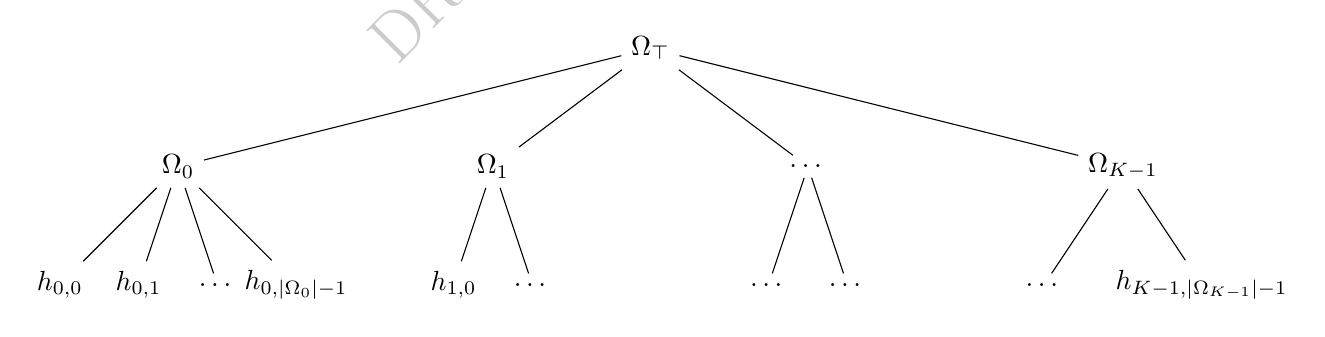
\begin{tikzpicture}
\node {\(\Omega_\top\)} [sibling distance = 4cm]
  child {node {\(\Omega_0\)}  [sibling distance = 1cm]
    child {node {\(h_{0, 0}\)}}
    child {node {\(h_{0, 1}\)}}
    child {node {\dots}}
    child {node {\(h_{0, |\Omega_0| - 1}\)}}
  }
  child {node {\(\Omega_1\)}  [sibling distance = 1cm]
    child {node {\(h_{1, 0}\)}}
    child {node {\dots}}  
  }
  child {node {\dots}  [sibling distance = 1cm]
    child {node {\dots}}
    child {node {\dots}}
  }
  child {node {\(\Omega_{K-1}\)}   [sibling distance = 2cm]
    child {node {\dots}}
    child {node {\(h_{K-1, |\Omega_{K-1}| - 1}\)}}
  };
\end{tikzpicture}

Now let \(\Omega\) be the set of all outcomes \(\Omega_0 \cup \Omega_1 \cup \dots \Omega_{K-1}\). We can create a new RPF - just called \(P\) acting on \(\Omega\) - with the following assumptions:

1) If the two outcomes fall under the same component, then their relative probabilities do not change:

\begin{equation}
\label{rpf_composition_same_branch}
P(h_{k, i}, h_{k, j}) = P_k(h_{k, i}, h_{k, j})
\end{equation}

2) If the two outcomes fall under different components, then their relative probabilities are given as follows.

\begin{equation}
\label{eq:rpf_composition_different_branch}
P(h_{k_1, i}, h_{k_2, j}) = P_{k_1}(h_{k_1, i}, \Omega_{k_1}) \cdot  P_{\top}(\Omega_{k_1}, \Omega_{k_2}) \cdot P_{k_2}(\Omega_{k_2}, h_{k_2, j})
\end{equation}

Note the use of the composition property to traverse up and down the tree. One could of course imagine this for a tree being many levels, and having a different height for each branch.

\begin{theorem}
\(P\) respects the fundamental axioms.
\end{theorem}

\begin{proof}
Identity is obvious because an outcome is on the same component as itself, so we can use equation \ref{rpf_composition_same_branch} to get \(P(h_{k, i}, h_{k, i}) = P_k(h_{k, i}, h_{k, i}) = 1\)

The inverse and composition laws must be true if both inputs are in the same component, because that component already follows the axioms. We not assume that the two inputs are from different components.

The inverse law can be proven by calculation.
\begin{equation}
\begin{aligned}
P(h_{k_1, i}, h_{k_2, j})^{-1} &= (P_{k_1}(h_{k_1, i}, \Omega_{k_1}) \cdot  P_{\top}(\Omega_{k_1}, \Omega_{k_2}) \cdot P_{k_2}(\Omega_{k_2}, h_{k_2, j}))^{-1} \\
& = P_{k_1}(h_{k_1, i}, \Omega_{k_1})^{-1} \cdot  P_{\top}(\Omega_{k_1}, \Omega_{k_2})^{-1} \cdot P_{k_2}(\Omega_{k_2}, h_{k_2, j})^{-1} \\
& = P_{k_1}(\Omega_{k_1}, h_{k_1, i}) \cdot  P_{\top}(\Omega_{k_2}, \Omega_{k_1}) \cdot P_{k_2}(h_{k_2, j}, \Omega_{k_2}) \\
& = P_{k_2}(h_{k_2, j}, \Omega_{k_2})\cdot  P_{\top}(\Omega_{k_2}, \Omega_{k_1}) \cdot P_{k_1}(\Omega_{k_1}, h_{k_1, i}) \\
& = P(h_{k_2, j}, h_{k_1, i})
\end{aligned}
\end{equation}

Composition can be shown similarly - now naming the 3 separate indecies in components \(k_1, k_2, k_3\) as \(i_1, i_2, i_3\) respectively.
\begin{equation}
\begin{aligned}
& P(h_{k_1, i_1}, h_{k_2, i_2}) \cdot P(h_{k_2, i_2}, h_{k_3, i_3}) \\
& :\cong P_{k_1}(h_{k_1, i_1}, \Omega_{k_1}) \cdot  P_{\top}(\Omega_{k_1}, \Omega_{k_2}) \cdot \textcolor{red}{P_{k_2}(\Omega_{k_2}, h_{k_2, i_2}) \cdot  P_{k_2}(h_{k_2, i_2}, \Omega_{k_2})} \cdot  P_{\top}(\Omega_{k_2}, \Omega_{k_3}) \cdot P_{k_3}(\Omega_{k_3}, h_{k_3, i_3}) \\
& :\cong P_{k_1}(h_{k_1, i_1}, \Omega_{k_1}) \cdot  \textcolor{red}{P_{\top}(\Omega_{k_1}, \Omega_{k_2}) \cdot  P_{\top}(\Omega_{k_2}, \Omega_{k_3})} \cdot P_{k_3}(\Omega_{k_3}, h_{k_3, i_3}) \\
& :\cong P_{k_1}(h_{k_1, i_1}, \Omega_{k_1}) \cdot  P_{\top}(\Omega_{k_1}, \Omega_{k_3}) \cdot P_{k_3}(\Omega_{k_3}, h_{k_3, i_3}) \\
& :\cong P_{k_1}(h_{k_1, i_1}, h_{k_3, i_3})
\end{aligned}
\end{equation}
\end{proof}

\begin{theorem}
\(P\) is totally comparable if and only if the following are true:

\begin{enumerate}
\item \(P_{\top}\) is totally comparable
\item For all \(k \in \{0, 1, ..., K - 1\}\), \(P_k\) is totally comparable
\item There is at most one component with outcomes that are impossible with respect to that component. Equivalently, if \(h_{k_1, i}\) and \(h_{k_2, j}\) are two components, and \(P_{k_1}(h_{k_1, i}) = P_{k_2}(h_{k_2, j}) = 0\), then \(k_1 = k_2\). Also equivalently, all components except at most one are totally mutually possible.
\item If there is one component with outcomes that are impossible with respect to that component, then no element of \(P_{\top}\) is impossible with respect to that component.
\end{enumerate}
\end{theorem}

\begin{proof}
If all the components are totally comparable, then we only need to prove that outcomes in different components are comparable. Starting with equation \ref{eq:rpf_composition_different_branch},

\begin{equation}
P(h_{k_1, i}, h_{k_2, j}) = P_{k_1}(h_{k_1, i}, \Omega_{k_1}) \cdot  P_{\top}(\Omega_{k_1}, \Omega_{k_2}) \cdot P_{k_2}(\Omega_{k_2}, h_{k_2, j})
\end{equation}

The right hand side of the equation doesn't have any wildcards in it, so the only way that it can end up being \(= \ast\) is if there are both \(0\) and \(\infty\) as factors.

Because there is at most one component with outcomes impossible with respect to that component, we can say that either \(P_{k_1}(h_{k_1, i}, \Omega_{k_1}) = 0\) or \(P_{k_2}(h_{k_2, j}, \Omega_{k_2}) = 0\), or possibly neither, but not both.

Also, neither can be \(\infty\) [MAKE LEMMA].

If neither is 0, then the right hand side cannot be \(\infty\)

If the first term is 0, then the only way the entire right hand side can be \(\ast\) is if \(P_{\top}(\Omega_{k_1}, \Omega_{k_2}) = \infty\). But this can't be true because that would make \(\Omega_{k_2}\) impossible with respect to \(\Omega_{k_1}\), the sole component with impossible outcomes!

An analogous argument can be made if \(P_{k_2}(h_{k_2, j}, \Omega_{k_2} = 0\).

Therefore, the right hand side of the equation is not \(ast\) and \(P\) is totally comparable.

In the opposite direction, we can show that if any of the conditions are broken, then \(P\) is not totally comparable. Breaking any of the first two conditions would introduce an explicit \(\ast\) into equation \ref{eq:rpf_composition_different_branch}. If there are multiple components with impossible outcomes, then it would introduce a \(0\) into the first term of equation \ref{eq:rpf_composition_different_branch} and an \(\infty\) into the third term, yielding \(\ast\).

And finally, if only the fourth condition is broken, it would introduct a 0 into the first term of equation \ref{eq:rpf_composition_different_branch} and an \(\infty\) into the \textbf{second} term of equation \ref{eq:rpf_composition_different_branch}.

Therefore, if any of these conditions are broken, \(P\) is \textbf{not} totally comparable.
\end{proof}

\section{Bayesian Inference on Relative Distributions}

A relative probability function represents a belief over the set of potential hypotheses in \(\Omega\).

Start with the Bayesian inference formula for conditional probability for \(h \in \Omega\) assuming that we recieve data \(D\).

\[P(h|D) = \frac{P(D|h) \cdot P(h)}{P(D)} \qquad P(D) = \sum_{h \in \Omega} P(D|h) \cdot P(h)\]

Now we convert to relative probability by looking at the ratio between the two hypotheses.

\[\frac{P(h_1|D)}{P(h_2| D)} = \frac{P(D|h_1) \cdot P(h_1)}{P(D)} \div \frac{P(D|h_2) \cdot P(h_2)}{P(D)} = \frac{P(D|h_1) \cdot P(h_1)}{P(D|h_2) \cdot P(h_2)} \]

Notice that each component is represented by a ratio. By making the appropriate subsitutions, we can express this entirely in terms of relative probability functions.

For the ratio of prior probabilities, substitute the relative prior: \(\frac{P(h_1)}{P(h_2)} \rightarrow P(h_1, h_2) \)

For the ratio of posterior probabilities, substitute the relative posterior: \(\frac{P(h_1|D)}{P(h_2|D)} \rightarrow P(h_1, h_2|D) \)

It is more difficult to see that the likelihood ratio is a relative probability, but the Kolmogorov definition to expand conditional probability suggests that it is:

\[\frac{P(D|h_1)}{P(D|h_2)} = \frac{\frac{P(D \cap h_1)}{P(D)}}{\frac{P(D \cap h_2)}{P(D)}} = \frac{P(D \cap h_1)}{P(D \cap h_2)} \]

Therefore, we can let \(P_D\) represent the likelihood ratio of the different hypotheses, and we can be sure that it fits the RPF framework with regards to the fundamental axioms. The likelihood ratio \(P_D(h_1, h_2)\) encodes a description of how the different hypotheses rate the likelihood of data.

The substitution for the liklihood ratio is as follows: \(\frac{P(D|h_1)}{P(D|h_2)} \rightarrow P_D(h_1, h_2) \)

Now we get bayes rule for relative probability:

 \[P(h_1, h_2|D) = P_D(h_1, h_2) P(h_1, h_2)\]
 
Bayesian inference is not reduced to an element-by-element multiplication of two different RPFs: \(P_D(h_1, h_2)\) and \(P(h_1, h_2)\). Fortunately, product of two RPFs also obeys the fundamental axioms.

\begin{theorem} 
Let \(P_1\) and \(P_2\) be relative probability functions on \(\Omega\). Define \(P(h_1, h_2) = P_1(h_1, h_2) \cdot P_2(h_1, h_2)\). Then, \(P\) is also an RPF, that it is obeys the fundamental axioms.
\end{theorem}

\begin{proof} 
Use the multiplication property of the matching relation in equation \ref{theorem:matching_multiplication}.
 
Identity: \[P(h_1, h_1) = P_1(h_1, h_1) P_2(h_1, h_1)=1 \cdot 1=1\]
 
Inverse: \[P(h_1, h_2) = P_1(h_1, h_2) \cdot P_2(h_1, h_2)=P_1(h_2, h_1)^{-1} \cdot P_2(h_2, h_1)^{-1}=(P_1(h_2, h_1) \cdot P_2(h_2, h_1))^{-1}=P(h_2, h_1)^{-1}\]
 
Composition: \[P(h_1, h_2)P(h_2, h_3)=P_1(h_1, h_2) P_2(h_1, h_2)P_1(h_2, h_3) P_2(h_2, h_3) :\cong P_1(h_1, h_3) P_2(h_1, h_3)=\]
\end{proof}

\begin{theorem}
Once two outcomes become uncomparable, they will never be comparable again. In other words, if \(P(h_1, h_2)=\ast\), then \(P(h_1, h_2|D) = \ast\).
\end{theorem}

\begin{proof}
\(P(h_1, h_2|D) = L(D|h_1, h_2) P(h_1, h_2) = P_D(h_1, h_2) \cdot \ast = \ast\)
\end{proof}

\begin{theorem}
Once an outcome becomes impossible with respect to another event, it will either remain impossible or become uncomparable. In other words,  if \(P(h_1, h_2)=0\), then \(P(h_1, h_2|D) \in {0, \ast}\).
\end{theorem}

\begin{proof}
\(P(h_1, h_2|D) = L(D|h_1, h_2) P(h_1, h_2) = P_D(h_1, h_2) \cdot 0\). Normally, this would simplify to 0, but with the matching relation in \(\mathbb{M}^*\), this will be \(\ast\) if \(P_D(h_1, h_2) \in {\infty, \ast}\).
\end{proof}

\section{Implementation}

Finally, we implement relative probabiliy as a python class as a demonstration of its usage and relevance.

How to implement this in code, and point to open source example.

Note the connection between magnitude space and the extended real number line, which we can implement through floating point numbers.

This can be implemented by storing K values.

For each category, we have a tier. Items in the same tier are comparable. Each Tier has a parent tier, where items in this teir are said to be impossible relative to anything in its ancestor tiers.

For each category, we also store a floating point number called the value, which should be taken as the log of an unnormalized probability. Note that we will not allow inf or NaN here.

Get the relative probability of 2 categories. Algorithm: If they are in the same tier, then subtract their values and take the exp. If they are in different tiers, do a graph search on the tier. If the first is < the second, the answer is 0. If the first is > the second, the answer is 1. And if they are uncomparable, then the answer is Wildcard, NaN.

Generate and indifferent distribution of category K. Algorithm: Create a single tier where all values are set to 0.

Change the relative probability of item \(k_1\) with respect to \(k_2\), and set it to \(q\). Algorithm: UNSURE

Set the probability \(k_1\) to some absolute value with respect to either the whole distribution, or to its tier.

Randomly sample from this distribution. Algorithm: Only look at the top tier.

Randomly sample from this distribution, but remove certain categories. Algorithm: If the top tier categories are gone, look to see if a top tier remains. If there are multiple top tiers, then there's no way to do it!

Ask: Is this distribution totally mutually possible? Algorithm: Look are a single top tier.

Ask: Is it totally comparable? Algorithm: Look for a linear list of tiers.

\section{Topology of Relative Probability Spaces}

\begin{definition}
\(\Omega\) is a set of outcomes. Define \(\text{RPF}^{\ast}(\Omega)\) as the set of relative probability functions on \(\Omega\). Likewise, define \(\text{RPF}(\Omega)\) as the set of all totally comparable RPFs. 
\end{definition}

Mathematics can be great at modelling the real world even through ideas that are theoretically impossible. For example, we might believe that it is impossible for a certain natural process to repeat an infinite number of times, and yet we may still take its value to be infinity in order to get some kind of bound on what that system will look like in the long run. Likewise, it still makes sense to consider a particular outcome in a probabilistic system as certain while maintaining information about the other outcomes in order to calculate the effects of such a limit. One of the benefits of relative probability spaces is their properties with respect to limits. To this end, we will prove that when we take limits of totally mutually comparable RPFs, the resulting RPF will also be titally mutually comparable.

If we look at the space of (absolute) categorical distributions on \(\Omega\) and we allow the probability of one outcome to approach 1, then all of the other probabilities will be forced down to 0 and become incomparable with one another. In the relative probability space, the information about the ratios of probabilities of the other outcomes can be preserved even as a single outcome reaches a probability of 1.

TODO: Warn people that background in topology is required for this section, and then we can shorten it up! Also, this section can be skipped if not interesting.

If the space of totally comparable RPFs is compact, then information about the relative probabilites of events are preserved even as they approach zero relative to another event.

In order to prove compactness, we first must define a topology on the space of totally comparable RPFs. This means identifying the open sets.\footnote{This author finds it useful for intuition to think of an open set as a set that fully surrounds all of it's members and therefore does not contain a boundary.}. This starts with finding a \textit{basis of open sets} from which all other open sets can be constructed through intersections and countable unions.

For the absolute probability function, we can use a \(K-1\)-simplex embedded in \(\mathbb{R}^K\) to get a topology using the standard Euclidean space. This strategy fails for relative probabilities, because there is no obvious way to embed an RPF into euclidean space\footnote{Though it may be possible! See section \ref{section:euclidean_embedding}}.

The notion of an open set can change even if a topological space is restricted. For example, on the real number line \(\mathbb{R}\), we take the open interval (0, 1) as an open set (as the term open interval suggests). However, once this is embedded into \(\mathbb{R}^2\), it is now a line segment in a plane and no longer open. It can be thought of as a restriction to an open set on \(\mathbb{R}^2\) to \(\mathbb{R}\). For example, the set \(\{(x, y): x \in (0, 1)\;  \text{and}\;  y \in (-\epsilon, +\epsilon)\}\) given an \(\epsilon > 0\) is such an open set on \(\mathbb{R}^2\). [ILLUSTRATION]

Likewise, an open set on a relative probability space restricted on several outcomes might not be an open set on the relative probability spaces for all of \(\Omega\).

We start by looking at RPFs with \(K = 2\). Fortunately, we find a totally comparable RPF that corresponds 1:1 with the magnitude space.

\begin{theorem}
Let \(\Omega = \{h_1, h_2\}\) have two elements, with relative probability function \(P\). Then, \(P\) is completely determined by \(P(h_1, h_2)\).
\end{theorem}

\subsection{Open Patches}

We now develop a notion of open patches, which will be a bases of open sets on the space \(\text{RPF}_{\text{comp}}(\Omega)\).

\begin{proof}
Let \(q = P(h_1, h_2)\). By the inverse symmetric property, \(P(h_2, h_1) = q^{-1}\). These values completely determine \(P\) on the event level.
\end{proof}

\begin{corollary}
The space of RPFs with \(K = 2\) corresponds 1:1 with \(\mathbb{M}^*\), and the space of totally mutually comparable RPFS corresponds to \(\mathbb{M}\)
\end{corollary}

\begin{definition}
An \textit{interior open patch} of \(\text{RPF}_{\text{comp}}(\Omega)\) is one of the following:

\begin{enumerate}
  \item If \(K = 2\), a subset parameterized by an interior open interval of magnitudes. \(\{P | a < P(h_1, h_2) < b\}\) for some \(a, b \in \mathbb{M}\) 
  \item If \(K > 2\), a composition of interor patches with composing function \(P_{\top}\) also being an interior patch.
\end{enumerate}
\end{definition}

Intuition: Interior open patches contain only totally mutually possible functions. (should this be a theorem?)

Insert: diagram for interior open patches

\begin{definition}
A \textit{facet patch} of \(\text{RPF}_{\text{comp}}(\Omega)\) is one of the following:

\begin{enumerate}
  \item If \(K = 2\), an interval of the form \(\{P | 0 < P(h_1, h_2) < a\}\) for some \(a \in \mathbb{M}\) 
  \item If \(K > 2\), the set of compositions where \(P_{\top}\) is drawn from an interior open patch, and all but one of the components are drawn from interior open patches. The last component - called the \textit{facet component} is itself a facet patch.
\end{enumerate}
\end{definition}

Insert: diagram for facet patches

Definition: An \textit{exterior open patch} is a one of the following:

\begin{enumerate}
  \item Any facet patch is also and exterior open patch
  \item A composition where \(P_{\top}\) is a facet patch. The \textit{facet component} is itself drawn from an exterior open patch, and all the other components are drawn from interior open patches.
\end{enumerate}

Intuition: Exterior open patches contain only totally mutually comparable functions, but some are not totally mutually possible.

Insert: diagram for exterior open patches

TODO: Break this down because it's not that intuitive!

Definition: An \textit{open patch} is a subset of \(\text{RPF}_{\text{comp}}(\Omega)\) that is either an interior or exterior open patch.

Every element of an open patch of \(\text{RPF}(\Omega)\) is totally mutually comparable.

Now let the open patches be the bases for an open set thus defining a topology on the set of totally mutually comparable RPFs of \(\Omega\).

\begin{definition}
Let the set of open patches define a basis for the topology on \(\text{RPF}_{\text{comp}}(\Omega)\).
\end{definition}

\subsection{Compactness}

\begin{theorem}
The topological space of totally comparable functions on an outcome space \(\Omega\) is \textit{compact}, meaning that for every open cover of it, there is a finite subcover.
\end{theorem}

\begin{proof}
STILL A LOT TO DO:

Let \(K = |\Omega|\). This is going to be an inductive proof where we assume that the theorem is true for all \(k < K\) and then prove that it is true for \(K\).

If \(K \in {0, 1}\) then the set of open sets is finite, so we're good. (Reference degenerate cases)

Let \(h \in \Omega\) be an outcome. The space of totally comparable functions on \(\Omega\) can be split into 2 regions: one where \(P(h, \Omega) = 0\) and one where \(P(h_1, \Omega) > 0\).

- We're going to have to prove this - might be tough!
\end{proof}

\subsection{Simple Limit Example}

Let us define a simple relative probability distribution \(P_q\) where \(K = 3\) that is parameterized by the magnitude \(q \in \mathbb{M}\).

Let \(P_q(h_0, h_1) = q\) and \(P_q(h_1, h_2) = 2\).

By the fundamental property, \(P_q(h_0, h_2) :\cong P_q(h_0, h_1) \cdot P_q(h_1, h_2) = 2q\).

Now we want to consider the case where the relative probability of \(h_0\) grows infinitely large in comparison to \(h_1\) and \(h_2\).

\[P = lim_{q \rightarrow \infty} P_q\]

We use the following topological definition for the limit in this case: For every open set A of relative probability distributions containing P, there exists an open interval \(B=(b, \infty)\) on \(\mathbb{M}\) such that for every value of \(q \in B\), \(P_q\) is in A.

\begin{proposition}
The above limit that defines \(P\) exists, and \(P(h_1, h_2) = 2\). In other words, \(h_2\) is still half as likely as \(h_1\) and that information hasn't been lost on \(P\).
\end{proposition}

\begin{proof}
TODO
\end{proof}

\section{Future Work}
\subsection{Expansions to infinite spaces}
- Including topological and metric
- Much richer world, more complex mathematics, more applications
- Is it possible to create a univified version of the Hausdorff measure, where objects are categorized by dimention \(d\), and a smaller-dimentional object is always mutually impossible to a larger dimentional object.
\subsection{Connection Surreal Numbers}
- This is greater, richer than the real number system
- Does this abrograte the need for the relative probability function (not for incomparable values)
- If the infinite case is dealt with above, then more questions are raised about both the power of surreal numbers and their suitability
\subsection{Shrinking the Measure Number System}
- We still have a usable system if we want Rational Numbers
- Can this system work for all non-standard probability value systems?
- There is practical application in this work, since computers cannot work with real numbers directly. We implement this system with floating point numbers and this approximation should be good enough for most applications - but can we have a version with more precise arithmetic
\subsection{Relationship to Category Theory}

Category theorists will instantly recognize that an RPF describes a category perfectly. This construction can be analyzed and approached through the lens of category theory.

The recent work of Censi et al.\cite{censi} concerns negative information in categories, which here corresponds to the wildcard element. It represents regions of the probability function that remain unassigned or uncomparable. This work could be used to subsume and further develop the idea of the wildcard.
\subsection{Embedding in Euclidean Space}
\label{section:euclidean_embedding}
FILL IN
Hexagon diagram
\begin{appendices}

\section{Is an Appendix Needed}

\end{appendices}

%\subsubsection*{References}

\begin{thebibliography}{20}

\bibitem{sklar_dirichlet}Sklar, M. (2014). Fast MLE computation for the Dirichlet multinomial. arXiv preprint arXiv:1405.0099.
\bibitem{sklar_bias}Sklar, M. (2022). Sampling Bias Correction for Supervised Machine Learning: A Bayesian Inference Approach with Practical Applications. arXiv preprint arXiv:2203.06239.
\bibitem{mendelson}Mendelson, B. (1990). Introduction to topology. Courier Corporation.
\bibitem{bradley}Bradley, T. D., Bryson, T., \& Terilla, J. (2020). Topology: A Categorical Approach. MIT Press.
\bibitem{lyon}Lyon, A. (2016). Kolmogorov’s Axiomatisation and its Discontents. The Oxford handbook of probability and philosophy, 155-166.
\bibitem{hajek}Hájek, A. (2003). What conditional probability could not be. Synthese, 137(3), 273-323.
\bibitem{censi}Censi, A., Frazzoli, E., Lorand, J., \& Zardini, G. (2022). Categorification of Negative Information using Enrichment. arXiv preprint arXiv:2207.13589.
\bibitem{ieee}Kahan, W. (1996). IEEE standard 754 for binary floating-point arithmetic. Lecture Notes on the Status of IEEE, 754(94720-1776), 11.
\bibitem{kolmogorov}A. N. Kolmogorov. Foundations of the Theory of Probability. Chelsea Publishing Company, New York
(1956). 

\end{thebibliography}

This document along with revisions is posted at github as https://github.com/maxsklar/relative-probability-finite-paper. See readme for contact information. Local Maximum Labs is an ongoing effort create an disseminate knowledge on intelligent computing.
\end{document}
